\chapter{Force-Guided Robot Alignment}
This chapter follows on from the previous chapter, we continue to demonstrate some technical solutions of system integration. On top of that, F/T sensor will be included to discuss. Therefore, you can see the chapter as a operating manual when you simultaneously own a robot arm, an F/T sensor and an end effector. First of all, we explain why we will use F/T sensor in our project in section \ref{sec:pro def}. Furthermore, we introduce how to do gravity compensation in senction \ref{sec:grav compen}. Admittance control based on F/T sensor is described in section \ref{sec:adm ctrl}. Reference Frame Changing of F/T sensor is explained in section \ref{sec:rfc}. And finally we discuss affection of setting admittance control parameters in section \ref{sec:affection}.
\section{Problem Definition}
\label{sec:pro def}
(Main cause of surgical failure)
(Peg in hole method based on F/T feedback)
(Modes: Doctor Dragging and self-alignment)
how to compensate the gravity affection in section \ref{sec:grav compen}; how to use admittance control in section with F/T sensor \ref{sec:adm ctrl}; and how to obtain the real force and torque values in the tool tip frame in section \ref{sec:rfc}
\section{Integration of F/T sensor}
\label{sec:grav compen}
Gravity compensation is a standard technical issue when combining an F/T sensor, a robot arm and an end effector.
\section{Alignment to the Root Canal (Dragging for alignment)}
\subsection{Admittance Control based on F/T sensor}
\label{sec:adm ctrl}
Admittance control make the robot move like a spring-mass-damper system. Forces and torques can be mapped into the movements such as position or velocity. Therefore, Admittance control allows an robot arm to cooperate with human in a safe work environment. In this section we propose a control scheme depicted as Figure \ref{fig:adm ctrl}.
\begin{figure}[htbp]
\begin{center}
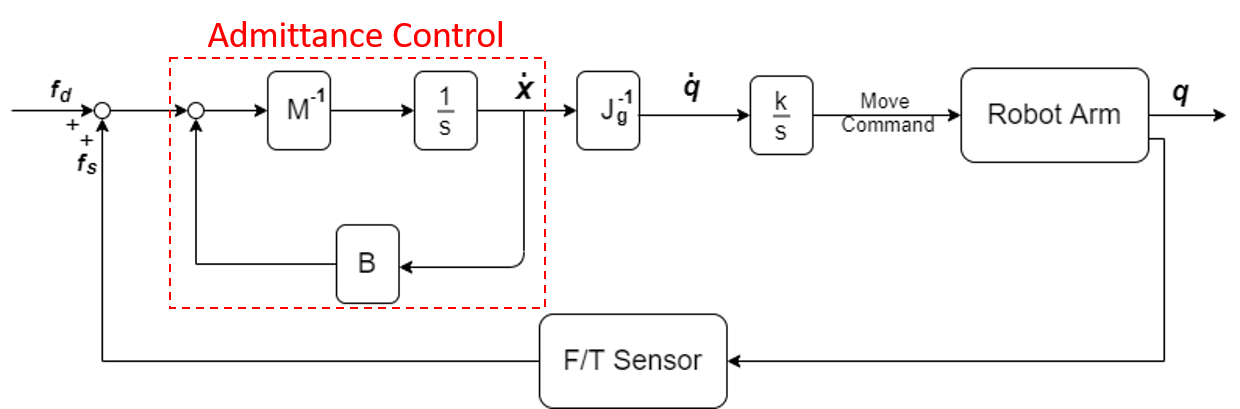
\includegraphics[width=1\linewidth]{Images/adm ctrl.png}
\end{center}
\caption{
Control scheme. Where $\text{F}_{\text{d}}$ denotes the desired forces and torques vector. $\text{F}_{\text{s}}$ denotes the real value detected by F/T sensor and is also a forces and torques vector. $\dot{\textbf{x}}$ denotes [$\dot{x}, \dot{y}, \dot{z}, \dot{\theta _x}, \dot{\theta _y}, \dot{\theta _z}$]. $\text{J}_{\text{g}}$ denotes the geometric Jacobian matrix. $\dot{\textbf{q}}$ denotes [$\dot{\theta _1}, \dot{\theta _2}, \dot{\theta _3}, \dot{\theta _4}, \dot{\theta _5}, \dot{\theta _6}$]. $\textbf{q}$ denotes [$\theta _1, \theta _2, \theta _3, \theta _4, \theta _5, \theta _6 $]
}\label{fig:adm ctrl}
\end{figure} 
Since Meca500 is an industrial robot arm without admittance control, we combine the robot arm with the F/T sensor to enable admittance control. With force and torque feedback, F/T sensor make Meca500 like a cooperative robot arm. It's worth noting that in this approach the admittance control function is triggered by the end effector mounted on F/T sensor instead of each wrist of the robot arm.\\
\begin{equation}
\label{eq:adm}
\begin{split}
\begin{bmatrix}
x \\
y \\
z \\
\theta _x \\
\theta _y \\
\theta _z \\
\end{bmatrix}
=
\frac{1}{MS^2+BS+K}
\begin{bmatrix}
f_x \\
f_y \\
f_z \\
\tau x \\
\tau y \\
\tau z \\
\end{bmatrix}
\end{split}
\end{equation}
where M,B,K are diagonal positive definite matrices. Affections of these parameters will be discussed in next section. \\
A standard equation of admittance control is represented as Eq \ref{eq:adm}. The values we obtain from the F/T sensor are $\left[f_x, f_y, f_z,\tau _x, \tau _y, \tau _z \right]$, whose forces $ \left[f_x, f_y, f_z\right]$ are related to the translations $ \left[x, y, z\right]$ and torques $ \left[\tau _x, \tau _y, \tau _z\right]$ are related to the axis angle $ \left[\theta _x,\theta _y,\theta _z\right]$. In our approach we ignore parameter $K$ which is relevant to spring stiffness because our system should behave like a mass-damper system. Bounce similar to a spring is not necessary in whole project. \\
There are few commands of moving the robot arm. Such as position command MoveJoints(\text{$\theta _1,\theta _2,\theta _3,\theta _4,\theta _5,\theta _6$})and MovePose(x,y,z,\text{$\alpha$} $\beta$ $\gamma$); velocity command MoveJointsVel\\
\section{Alignment to the Root Canal (Drilling and self-alignment)}
\subsection{Reference Frame Changing of F/T sensor}
\label{sec:rfc}
(Transformation from robot to tool [Chapt. 3.4]+ Transformation from sensor to tool) 
(How to find the direction vector of the tool)
(From sensor frame to tool tip frame)
\subsection{Motion Planning: Based on Admittance Control}
(Block diagram, robot command choice)
\section{Discussion about Affection of Parameter Setting}
\label{sec:affection}
(K, Bi, Mi- without numbers)
(Modes: Doctor Dragging and Self-alignment - with numbers; get reasonable and suitable parameters first)